\begin{frame}
  \frametitle{Artificial Neural Networks}
  \begin{itemize}
    \item Class of machine learning algorithms
      \begin{itemize}
        \item Loosely inspired by biological nervous systems
      \end{itemize}
    \item Collection of artificial neurons that are connected with
      each other
      \begin{itemize}
        \item Enables them to exchange signals along their connections
        \item Can be represented by a directed graph
      \end{itemize}
    \item Usually arranged in layers
      \begin{itemize}
        \item \textit{Input Layer} collects input signals and passes
          them on
        \item \textit{Hidden Layers} apply transformations to incoming
          signals and pass the outcomes further into the network
        \item \textit{Output Layer} applies a final transformation
          representing the networks' result
      \end{itemize}
    \item Goal: Convert input into meaningful output by applying
      multiple transformations
  \end{itemize}
\end{frame}

\begin{frame}
  \frametitle{Components of the neural model}
  \begin{itemize}
   \item A set of weighted inputs
     \begin{itemize}
       \item Each input originating from neuron \(j\) and traveling
         into neuron \(k\) is first multiplied by a weight \(w_{kj}\)
     \end{itemize}
   \item A summation unit
     \begin{itemize}
       \item All the weighted inputs are summed and a constant value,
         the \textit{bias}, is added to yield the result \(z_k\)
     \end{itemize}
   \item An activation function
     \begin{itemize}
       \item Applies a non-linear transformation \(\phi(\cdot)\) to
         the output of the summation unit
       \item This result, called \(y_k\), is propagated further into
         the network alongside the connections
     \end{itemize}
  \end{itemize}
\end{frame}

\begin{frame}
  \frametitle{The Role of the Bias Value}
  \begin{itemize}
    \item The bias is added as a constant to the sum of the weighted
      inputs in the summation unit
    \item Acts like a threshold that has to be overcome
      \begin{itemize}
        \item Negative bias: Positive weighted inputs needed for the
          neuron to become active
        \item Positive bias: Negative weighted inputs needed to stop
          the neuron from being active
      \end{itemize}
  \end{itemize}
\end{frame}

\begin{frame}
  \frametitle{The Role of the Bias Value}
  \begin{figure}
    \resizebox{.6\textwidth}{!}{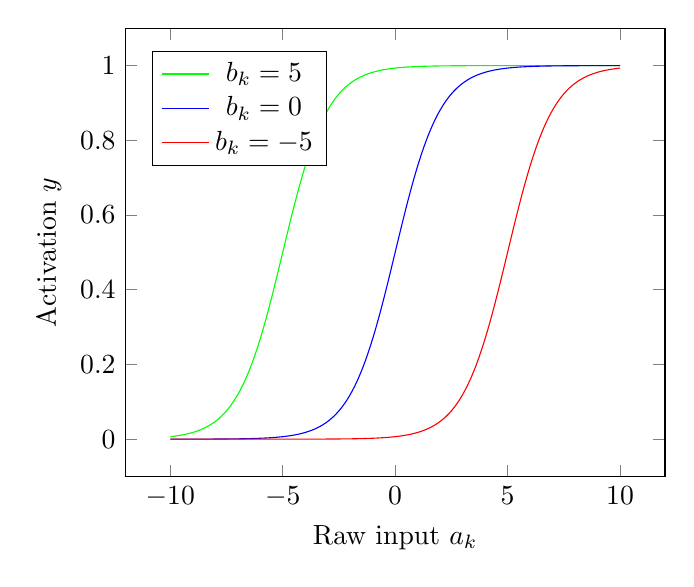
\begin{tikzpicture}
  \begin{axis}[
      xlabel={Raw input \(a_k\)},
      ylabel={Activation \(y\)},
      legend style={
        at={(0.05, 0.95)},
        anchor=north west
      }
    ]
    \addplot[green, domain=-10:10, samples=400]{1/(1+exp(-(x+5)))};
    \addplot[blue, domain=-10:10, samples=400]{1/(1+exp(-x))};
    \addplot[red, domain=-10:10, samples=400]{1/(1+exp(-(x-5)))};
    \legend{\(b_k = 5\), \(b_k = 0\), \(b_k = -5\)}
  \end{axis}
\end{tikzpicture}
}
    \caption{The sigmoid activation function plotted for different bias values.}
  \end{figure}
\end{frame}

\begin{frame}
  \frametitle{Evaluation Metrics}
  \begin{itemize}
    \item \textbf{Accuracy:}
      \begin{itemize}
        \item Percentage of testing examples that were classified correctly
      \end{itemize}
      \begin{equation}
        Accuracy = \frac{TP + TN}{TP + TN + FP + FN}
      \end{equation}
    \item \textbf{Precision:}
      \begin{itemize}
        \item Percentage of correctly classified examples among all
          examples classified as positive
      \end{itemize}
      \begin{equation}
        Precision = \frac{TP}{TP + FP}
      \end{equation}
  \end{itemize}
\end{frame}

\begin{frame}
  \frametitle{Evaluation Metrics}
  \begin{itemize}
    \item \textbf{Recall:}
      \begin{itemize}
        \item What percentage of positive examples was classified
          correctly?
      \end{itemize}
      \begin{equation}
        Recall = \frac{TP}{TP + FN}
      \end{equation}
    \item \textbf{F1 Score:}
      \begin{itemize}
        \item Harmonic mean of precision and recall
      \end{itemize}
      \begin{equation}
        \text{F1 Score} = \frac{2*Precision*Recall}{Precision+Recall}
      \end{equation}
  \end{itemize}
\end{frame}
